\documentclass[letterpaper,headings=standardclasses]{scrartcl}

\usepackage[margin=1in,includefoot]{geometry}
\usepackage{amssymb}
\usepackage{amsmath}
\usepackage{listings}
\usepackage{tikz}

\usetikzlibrary{shapes,arrows}

\tikzset{
  block/.style    = {draw, thick, rectangle, minimum height = 3em, minimum width = 3em},
  sum/.style      = {draw, circle},
  input/.style    = {coordinate, circle},
  output/.style   = {coordinate, circle}
}

\lstset{basicstyle=\ttfamily,language=python,columns=flexible,breaklines=true}

\title{Homework 1}
\subtitle{CS 559 - Neural Networks - Fall 2019}
\author{Matteo Corain 650088272}

\begin{document}

\maketitle

\section{Question 1}

\subsection{First logical product}

For the implementation of the first logical product $\bar{x_1} x_2 x_3$ in a perceptron, the standard design process can be followed; the only difference with the standard case stands in the output of the perceptron: in fact, since the signum activation function is used, this will be set to -1 to represent a logical false.

The first step is to compute the number $n$ of inputs that appear complemented in the logical product and the number $m$ of inputs that appear not complemented; in this case, we have $ n = 1 $ and $ m = 2 $. Given those values, we can proceed as follows:

\begin{itemize}

\item We assign a weight of 1 to all inputs that appear not complemented in the product;
\item We assign a weight of -1 to all inputs that appear complemented in the product;
\item We assign a weight of $-m + \frac{1}{2}$ to the perceptron's bias.

\end{itemize}

Using this procedure, we derive that a possible choice of weights that implements the requested logical function is:

$$ w_0 = -1 + \frac{1}{2} = -\frac{3}{2} $$
$$ w_1 = -1, w_2 = w_3 = 1 $$

\subsection{Second logical product}

The same process has been followed also for the implementation of the second logical product $ x_1 \bar{x_2} $; in this case, we have $ n = 1 $ and $ m = 1 $. A possible choice of weights that implements the requested logical function is:

$$ w_0 = -m + \frac{1}{2} = -\frac{1}{2} $$
$$ w_1 = 1, w_2 = -1, w_3 = 0 $$

\subsection{OR logical function}

For the implementation of the OR logical function, a custom design has been necessary since the two neurons in the first layer do not output, as usual, value 0 in case of false, but instead they output value -1. The single neuron in the second layer of the network, therefore, has to implement the logic function described by the following truth table:

\begin{table}[h]
\centering
\begin{tabular}{|c|c|c|}
\hline
$x_1$ & $x_2$ & $y$  \\ \hline
-1    & -1    & -1   \\ \hline
-1    & 1     & 1    \\ \hline
1     & -1    & 1    \\ \hline
1     & 1     & 1    \\ \hline
\end{tabular}
\caption{Truth table for the OR logical function using signum activation}
\end{table}

There are different approaches that can be followed for designing a neuron that implements this logic function. One of the simplest is a graphical procedure, based on the geometric interpretation of the perceptron. In fact, if we plot the four labeled data points on the $x_1$-$x_2$ plane, we can see that the two classes, yielding values -1 and 1, are clearly linearly separable. Thus, it is possible to identify a line that allows to separate the two classes; for example, a possible separator, shown in the figure, is described by the relation:

$$ 1 + x_1 + x_2 = 0 $$

\begin{figure}[h]
\centering
\includegraphics[width=.7\linewidth]{or_func.pdf}
\caption{Separator implementing the OR operator using signum activation}
\end{figure}

Remembering the general equation of a linear separator in a perceptron ($ w_0 + w_1x_1 + w_2x_2 = 0 $), a possible choice of weights that can be used to implement such a separator is:

$$ w_0 = w_1 = w_2 = 1 $$

This may also be analytically verified if we write the system of linear inequalities that describe this logical function; in fact, from the truth table we have that:

$$ \begin{cases} \text{sgn(} w_0 - w_1 - w_2 \text{)} = -1 \\ \text{sgn(} w_0 - w_1 + w_2 \text{)} = 1 \\ \text{sgn(} w_0 + w_1 - w_2 \text{)} = 1 \\ \text{sgn(} w_0 + w_1 + w_2 \text{)} = 1 \end{cases} \Rightarrow \begin{cases} w_0 - w_1 - w_2 < 0 \\ w_0 - w_1 + w_2 > 0 \\ w_0 + w_1 - w_2 > 0 \\ w_0 + w_1 + w_2 > 0 \end{cases} $$

It is simple to verify that the identified weights satisfy the four identified inequalities.

\subsection{Final network}

A possible network that implements the logical function $f(x_1,x_2,x_3) = \bar{x_1} x_2 x_3 + x_1 \bar{x_2}$, using the previously computed weights, is depicted in the figure below.

\begin{figure}[h]
\centering
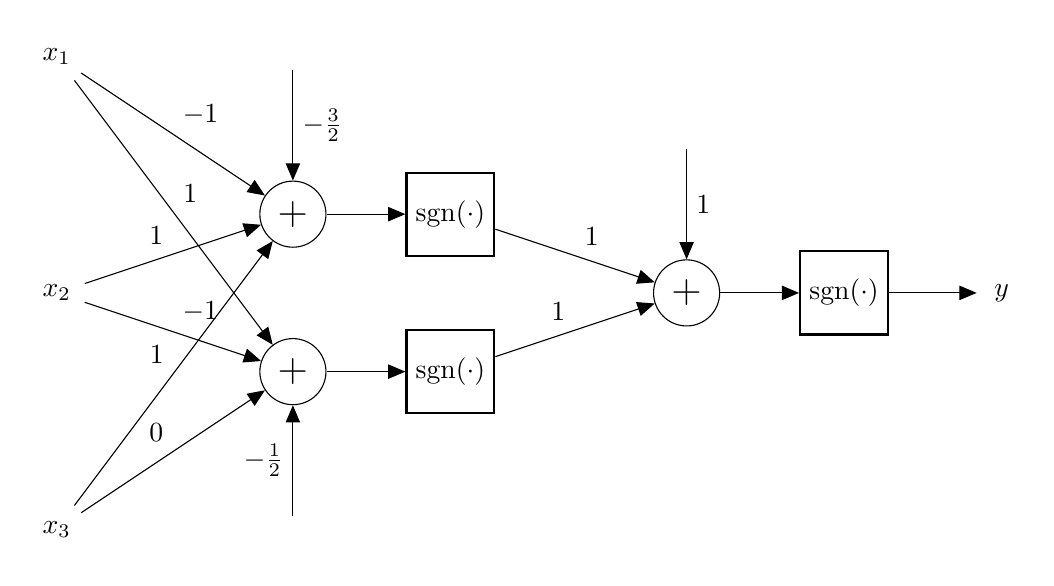
\begin{tikzpicture}[auto, node distance=2cm, >=triangle 45]

% Input layer
\draw node [input, name=x1] {$x_1$};
\draw node [input, name=x2, below of=x1, node distance=3cm] {$x_2$};
\draw node [input, name=x3, below of=x2, node distance=3cm] {$x_3$};

% First layer
\draw node [sum, right of=x2, yshift=1cm, node distance=3cm] (sum1) {\Large$+$};
\draw node [sum, below of=sum1] (sum2) {\Large$+$};
\draw node [input, name=x01, above of=sum1] {};
\draw node [input, name=x02, below of=sum2] {};
\draw node [block, right of=sum1] (act1) {sgn($\cdot$)};
\draw node [block, right of=sum2] (act2) {sgn($\cdot$)};

% Second layer
\draw node [sum, right of=act1, yshift=-1cm, node distance=3cm] (sum3) {\Large$+$};
\draw node [input, name=x03, above of=sum3] {};
\draw node [block, right of=sum3] (act3) {sgn($\cdot$)};
\draw node [output, name=y, right of=act3] {$y$};

% Connections
\draw[->](x01) -- node {$-\frac{3}{2}$}(sum1);
\draw[->](x1) -- node {$-1$}(sum1);
\draw[->](x2) -- node {$1$}(sum1);
\draw[->](x3) -- node {$1$}(sum1);
\draw[->](x02) -- node {$-\frac{1}{2}$}(sum2);
\draw[->](x1) -- node {$1$}(sum2);
\draw[->](x2) -- node {$-1$}(sum2);
\draw[->](x3) -- node {$0$}(sum2);
\draw[->](sum1) -- node {}(act1);
\draw[->](sum2) -- node {}(act2);
\draw[->](x03) -- node {$1$}(sum3);
\draw[->](act1) -- node {$1$}(sum3);
\draw[->](act2) -- node {$1$}(sum3);
\draw[->](sum3) -- node {}(act3);
\draw[->](act3) -- node {}(y);

\end{tikzpicture}
\caption{Final network that implements the given function}
\end{figure}

\section{Question 2}

\subsection{Analysis of the first layer}

In order to sketch the region in which the output of the network is $z = 1$, let's begin considering the first layer of neurons independently; for each of them, it is possible to write the input-output relationship, starting from the given weights:

\begin{itemize}

\item The first neuron implements the function $z_1 = u(1 + x - y)$, meaning that its output goes to 1 when $1 + x - y \ge 0 \Rightarrow y \le x + 1$;
\item The second neuron implements the function $z_2 = u(1 - x - y)$, meaning that its output goes to 1 when $1 - x - y \ge 0 \Rightarrow y \le -x + 1$;
\item The third neuron implements the function $z_3 = u(-x)$, meaning that its output goes to 1 when $-x \ge 0 \Rightarrow x \le 0$.

\end{itemize}

The regions in which the three neurons output a positive value can be represented on the $x$-$y$ plane as shown in the figure below.

\begin{figure}[h]
\centering
\includegraphics[width=\linewidth]{first_layer_out_sep.pdf}
\caption{Regions in which first layer neurons output a positive value}
\end{figure}

\subsection{Deduction of network output per region}

If we represent all those relationships on a single plane, then six different regions can be identified; each of those regions will represent a specific set of inputs of the second layer of the network. Analyzing those regions one by one, it is possible to deduce, for each of them, what will be the output of the network, given the input-output relationship of the second-layer neuron ($z = -1.5 + z_1 + z_2 - z_3$, where $z_1, z_2, z_3$ denote the outputs of the first-layer neurons):

\begin{enumerate}

\item In this region, the outputs of all first layer neurons is zero; therefore, the output $z$ of the neuron in the second layer is:

$$ z = u(-1.5 + 1 * 0 + 1 * 0 - 1 * 0) = u(-1.5) = 0 $$

\item In this region, the output of the first neuron is positive, while the outputs of the others are zero; therefore, the output $z$ of the neuron in the second layer is:

$$ z = u(-1.5 + 1 * 1 + 1 * 0 - 1 * 0) = u(-0.5) = 0 $$

\item In this region, the output of the first and second neurons are positive, while the output of the third is zero; therefore, the output $z$ of the neuron in the second layer is:

$$ z = u(-1.5 + 1 * 1 + 1 * 1 - 1 * 0) = u(0.5) = 1 $$

\item In this region, the outputs of all first layer neurons is positive; therefore, the output $z$ of the neuron in the second layer is:

$$ z = u(-1.5 + 1 * 1 + 1 * 1 - 1 * 1) = u(-0.5) = 0 $$

\item In this region, the output of the second and third neurons are positive, while the output of the first is zero; therefore, the output $z$ of the neuron in the second layer is:

$$ z = u(-1.5 + 1 * 0 + 1 * 1 - 1 * 1) = u(-1.5) = 0 $$

\item In this region, the output of the third neuron is positive, while the outputs of the others are zero; therefore, the output $z$ of the neuron in the second layer is:

$$ z = u(-1.5 + 1 * 0 + 1 * 0 - 1 * 1) = u(-2.5) = 0 $$

\end{enumerate}

\begin{figure}
\centering
\includegraphics[width=0.7\linewidth]{first_layer_out_all.pdf}
\caption{Combination of output regions of first layer neurons}
\end{figure}

The only region in which the network returns a positive value, therefore, is region number 3, including the separator of the second neuron (the blue line, on which the second neuron outputs $u(0) = 1$) but excluding the one of the third neuron (the green line, on which the third neuron outputs $u(0) = 1$). Graphically, it is possible to represent the two classes separated by this network on the $x$-$y$ plane as shown in the figure below; the dashed line indicates a zone for which $z = 0$, while the normal line a zone for which $z = 1$.

\begin{figure}[h]
\centering
\includegraphics[width=0.7\linewidth]{net_sep.pdf}
\caption{Classes separation using the given network}
\end{figure}

\section{Question 3}

\subsection{Exact weights selection}

The first steps of the problem require to generate a random vector of exact weights, which will be used later for the classification of the training samples. This has been accomplished by means of the \texttt{uniform()} function in the \texttt{random} library of the NumPy package; the generated weights have then been used to construct a Numpy \texttt{array} named \texttt{wr}. Those weights are then logged to the console; in this particular instance of the script, they were picked as:

$$ w_r = [\begin{matrix} -0.1437898 & 0.94758982 & 0.7844713 \end{matrix}] $$

\subsection{Generation of the training set}

The same approach has been used for the generation of the training set \texttt{S} for the network. This has been populated using the list comprehension syntax provided by the Python language, which allows to repeat the same action (in this case, the creation of a NumPy \texttt{array} having two randomly picked components) for a given number of times, described by the variable \texttt{n\_samples}. For convenience and efficiency, the training samples have been generated with an additional first component identically set to 1: this allows to multiply those vectors directly with a weights vector, taking into consideration also the contribution given by the perceptron's bias.

After the generation of the training set, the samples have been classified in two groups, \texttt{S0} and \texttt{S1}, according to the output returned by an “ideal” perceptron using the computed exact weights. For this purpose, the list comprehension syntax has been used again; in a first step, the vector of the desired outputs \texttt{d} has been computed, whose components are set to 1 in the case the result of the product $[ \begin{matrix}1 & x_1 & x_2 \end{matrix}][\begin{matrix} w_0 & w_1 & w_2 \end{matrix}]^T$ is positive, 0 otherwise. Using these data, the two sets \texttt{S0} and \texttt{S1} may be simply computed by considering the elements of the training set \texttt{S[i]} having respectively \texttt{d[i] = 0} or \texttt{d[i] = 1}. In this particular instance of the script, running with \texttt{n\_samples} equal to 100, we had 58 samples in set \texttt{S0} and 42 in set \texttt{S1}.

\subsection{Plotting data and separator}

\begin{figure}[h]
\centering
\includegraphics[width=.7\linewidth]{exact_sep.pdf}
\caption{Data separation using the exact weights}
\end{figure}

In order to plot the data and the ideal separator on the $x_1$-$x_2$ plane, the \texttt{plot\_data\_and\_sep()} function has been defined. This takes as parameters the two sets \texttt{S0} and \texttt{S1}, and the vector of weights \texttt{w} to be used. The function performs the following actions:

\begin{itemize}

\item It initializes a new Matplotlib figure;

\item It plots a data point for each element in set \texttt{S0}, using as its $x$ value its second component (the first is identically set to 1) and as its $y$ value its third component; data points in \texttt{S0} are represented by red squares;

\item It plots a data point for each element in \texttt{S1}, represented by blue circles;

\item It plots the separator line in dashed green, using as $x$ values -1 and 1 and as $y$ values the ones computed by expliciting the linear relationship for $x_2$ and substituting $x_1$ with -1 and 1:

$$ x_2 = -\frac{w_0 + w_1 x_1}{w_2} $$

\item It sets the boundaries of the figure to $[-1;1]$ along both axes;

\item It prints a title and a legend, then shows the result without blocking the execution.

\end{itemize}

\subsection{Running the Perceptron Training Algorithm}

The Perceptron Training Algorithm has been coded as a separate function, called \texttt{pta()}, which takes as argument the value of the parameter \texttt{eta} to be used, the vector \texttt{w0} of initial weights, the training set \texttt{S} and the vector of the desired outputs \texttt{d}. This function implements a slightly modified version of the standard PTA, performing the following actions:

\begin{itemize}

\item It initializes the PTA variables, creating a copy \texttt{w} of the array \texttt{w0} that will be used to compute the final weights and setting to 0 the number of \texttt{epochs} of the algorithm;

\item It initializes an array, called \texttt{mclass}, in which the number of misclassified objects is stored for each epoch (starting from epoch 0, which is the number of misclassifications computed using the initial random weights); those are computed using the \texttt{count\_mclass()} function, which sums inline the elements of a vector (created using the list comprehension syntax) whose components are set to 1 in case the value of the product $wx^T$ is different to the expected one, stored in the vector \texttt{d};

\item It starts a \texttt{while} loop, which stops when the number of misclassification at the previous epoch has reached zero (we have found the weights that correctly classify the entire training set); at each iteration:

\begin{itemize}

\item It increments the number of \texttt{epochs};

\item It loops through all training samples $x_i$, updating the weights according to the formula:

$$ w = w + \eta x_i (d_i - u(w x_i)) $$

\item It computes the number of misclassifications for the current epoch and logs the results.

\end{itemize}

\item When the main loop terminates, the procedure returns the array of the computed weights \texttt{w}, the number of \texttt{epochs} and the array of misclassifications per epoch \texttt{mclass}.

\end{itemize}

This function is made run multiple times with a variable value of \texttt{eta} but with a fixed vector \texttt{w0}, so that the differences in the results depend only on the selected value of the parameter. For this particular instance of the script, the obtained weights with the corresponding number of epochs needed for their computation are shown in the table below.

\begin{table}[h]
\centering
\begin{tabular}{|c|c|c|c|c|}
\hline
$\eta$ & $w_0$       & $w_1$       & $w_2$      & Epochs \\ \hline
1      & -0.6493862  & 4.58359584  & 3.94124711 & 7      \\ \hline
10     & -10.6493862 & 70.07911636 & 59.0983191 & 18     \\ \hline
0.1    & -0.1493862  & 0.86666667  & 0.67531926 & 21     \\ \hline
\end{tabular}
\caption{Computed weights using different values of $\eta$}
\end{table}

\subsection{Considerations on the computed weights}

Lorem ipsum dolor sit amet.

\subsection{Plotting the misclassification rate}

\begin{figure}[h]
\centering
\includegraphics[width=.7\linewidth]{mclass_per_epoch.pdf}
\caption{Number of misclassified items per epoch}
\end{figure}

After each run of the algorithm, the number of misclassified objects per epoch is plotted by means of the \texttt{plot\_mclass()} function; this performs the following actions:

\begin{itemize}

\item It initializes a new Matplotlib figure;

\item It plots the number of misclassification against the number of the epoch (epoch 0 represents the initial number of misclassified objects, using the random weights);

\item It adjust the axes of the graph (0 to the number of epochs for the $x$ axis, 0 to the maximum value of the misclassification vector for the $y$ axis);

\item It prints a title to the graph, enables the grid and shows the result without blocking the execution.

\end{itemize}

As expected, the number of misclassifications decreases with the epoch number, although not always monotonically, until it finally reaches zero (the desired weights have been computed).

\subsection{Effects of the value of $\eta$ on convergence speed}

Lorem ipsum dolor sit amet.

\subsection{Differences given by a larger number of samples}

Lorem ipsum dolor sit amet.

\subsection{Complete Python code}

\lstinputlisting[basicstyle=\ttfamily\scriptsize]{hw1_ex3.py}

\end{document}